\setcounter{section}{7}
\setcounter{subsection}{1}
\setcounter{figure}{5}
\begin{figure*}[t]
	\centering
	\begin{subfigure}{.39\linewidth}
		\centering
		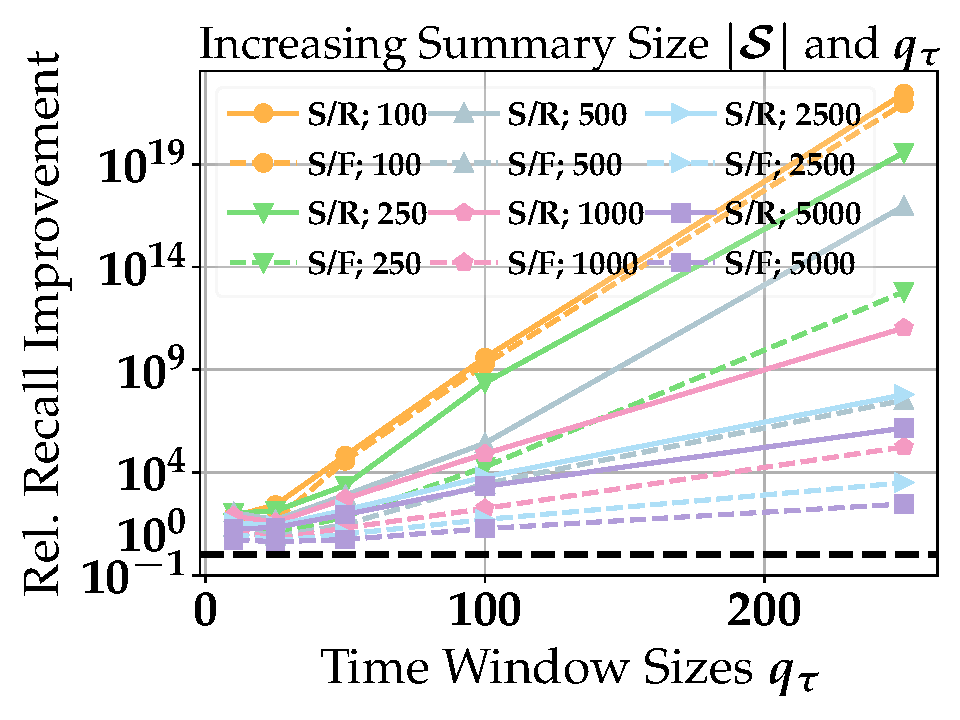
\includegraphics[width=\linewidth]{../runs/effectiveness/Figure6a_changing_summary_time_window_sizes/plots/summary_time_window_comparison.pdf}
		\vspace{-18pt}
		\caption{}
		\label{plot:summary_size_time_window_size}
	\end{subfigure}
	\hfill
	\begin{subfigure}{.39\linewidth}
		\centering
		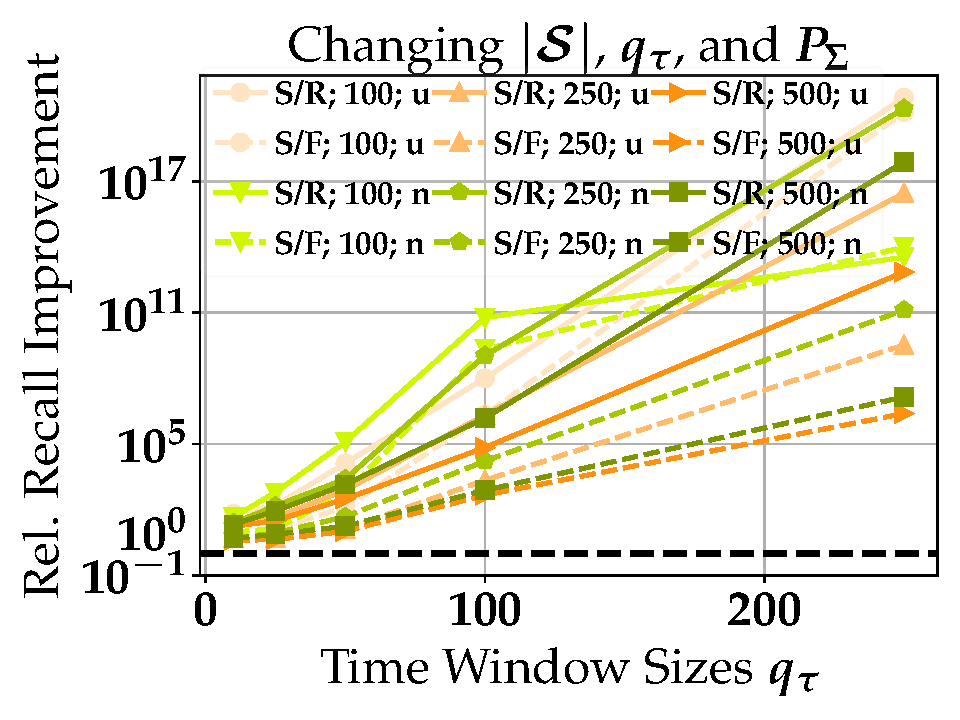
\includegraphics[width=\linewidth]{../runs/effectiveness/Figure6b_changing_probability_distribution/plots/probability_distribution_plot_uni_norm.pdf}
		\vspace{-18pt}
		\caption{}
		\label{plot:different_alphabet_probability_distributions}
	\end{subfigure}

	\vspace{-1em}
	\caption{Examining the impact on relative recall improvement (higher is better) by varying (a) summary and time window sizes and (b) the alphabet probability distribution $P_\Sigma$.}
	\label{fig:summary_size_time_window_size_evaluation_timestamps_query_length}
	\vspace{-1em}
\end{figure*}


\begin{figure*}[t]
	\centering
	\begin{subfigure}{.32\linewidth}
		\centering
		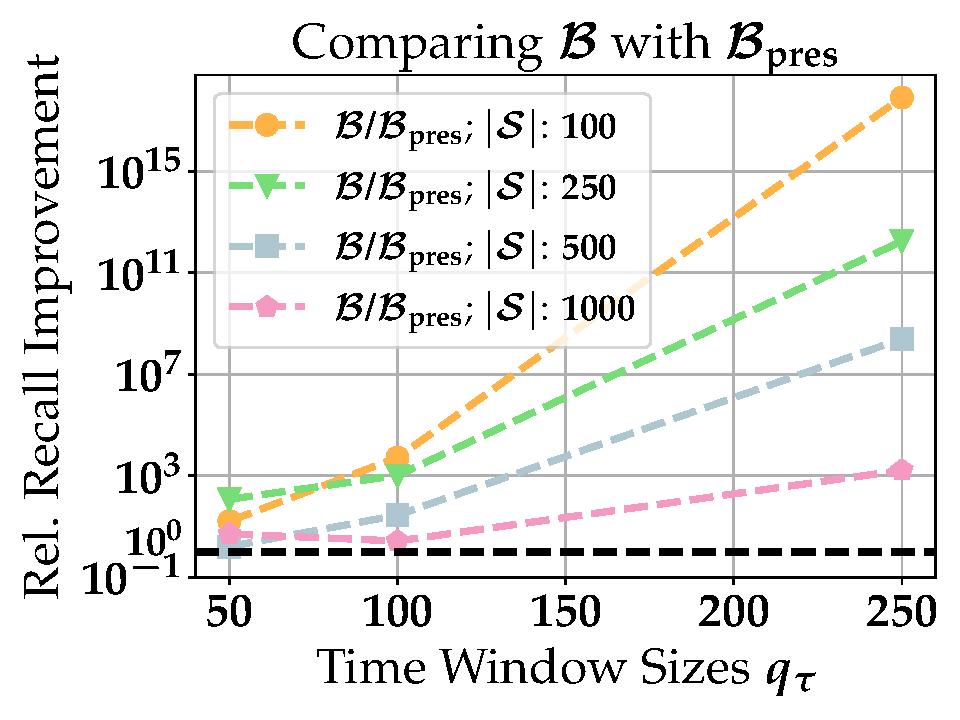
\includegraphics[width=1.0\linewidth]{../runs/effectiveness/Figure7a_ablation_study/plots/ablation_plot.pdf}
		\vspace{-18pt}
		\caption{}
		\label{plot:ablation_study}
	\end{subfigure}
	\begin{subfigure}{.32\linewidth}
		\centering
		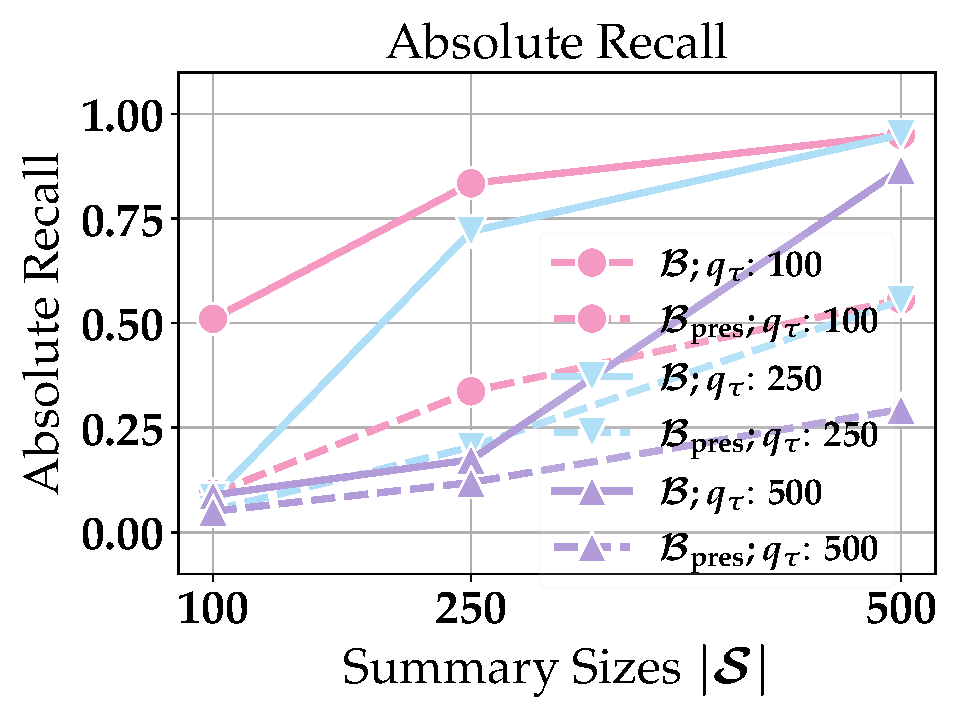
\includegraphics[width=1.0\linewidth]{../runs/effectiveness/Figure7b_total_matches_ratio_recall_stream_size_2000/plots/total_matches_ratio_recall_stream_size_2000.pdf}
		\vspace{-18pt}
		\caption{}
		\label{plot:average_total_match_ratio_recall_2000}
	\end{subfigure}
	\begin{subfigure}{.32\linewidth}
		\centering
		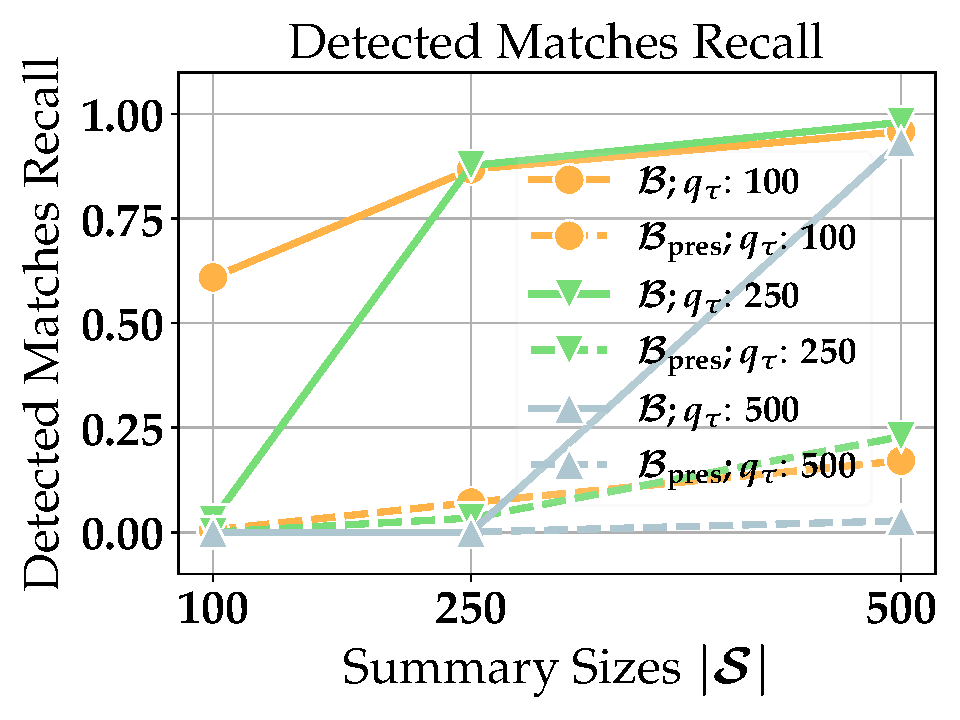
\includegraphics[width=1.0\linewidth]{../runs/effectiveness/Figure7c_detected_matches_recall_stream_size_2000/plots/detected_matches_recall_stream_size_2000.pdf}
		\vspace{-18pt}
		\caption{}
		\label{plot:detected_matches_recall_2000}
	\end{subfigure}
	\vspace{-1em}
	\caption{Examining the impact of the benefit function $\mathcal{B}$ compared to $\mathcal{B}_{\text{pres}}$ (a)
	on the relative recall improvement, (b) proximity to lower
	bound in absolute recall, and (c)
	proximity to lower bound in detected matches recall
	(higher is better in all plots).}
	\label{fig:ablation_study_and_recall}
	\vspace{-1em}
\end{figure*}


\begin{figure*}[t]
	\centering
	

	\begin{subfigure}{.38\linewidth}
		\centering
		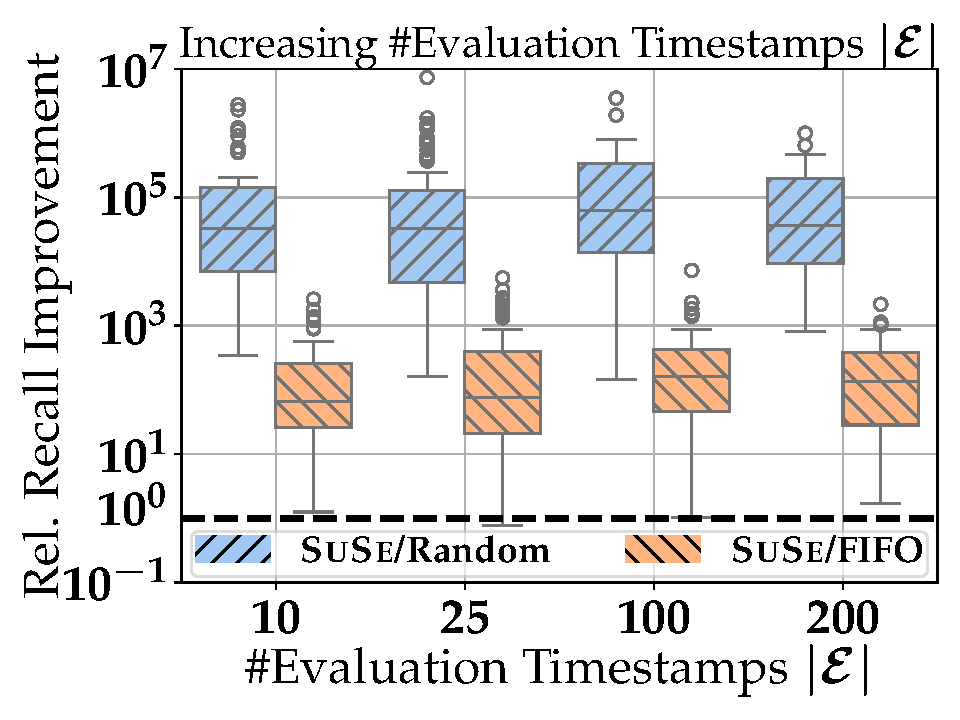
\includegraphics[width=\linewidth]{../runs/sensitivity_analysis/Figure8a_changing_number_of_eval_timestamps/plots/number_of_evaluation_timestamps_plot.pdf}
		\vspace{-18pt}
		\caption{}
		\label{plot:evaluation_timestamps}
	\end{subfigure}
	\hfill
	\begin{subfigure}{.38\linewidth}
		\centering
		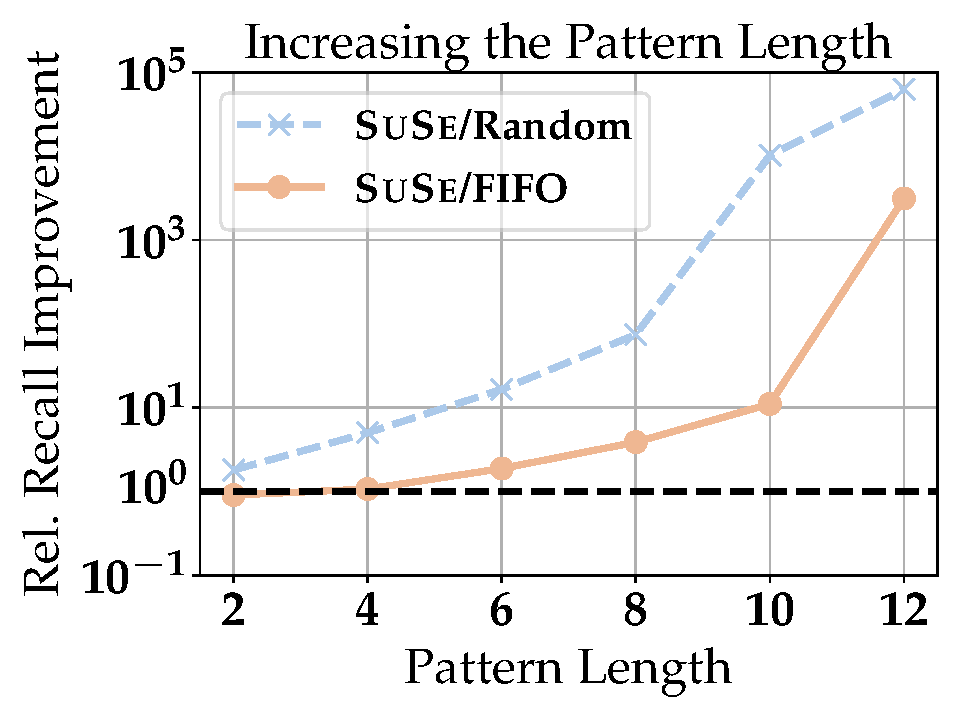
\includegraphics[width=\linewidth]{../runs/sensitivity_analysis/Figure8b_changing_query_length/plots/query_length_plot.pdf}
		\vspace{-18pt}
		\caption{}
		\label{plot:query_length}
	\end{subfigure}
    
    \vspace{1em} 
	\begin{subfigure}{.38\linewidth}
		\centering
		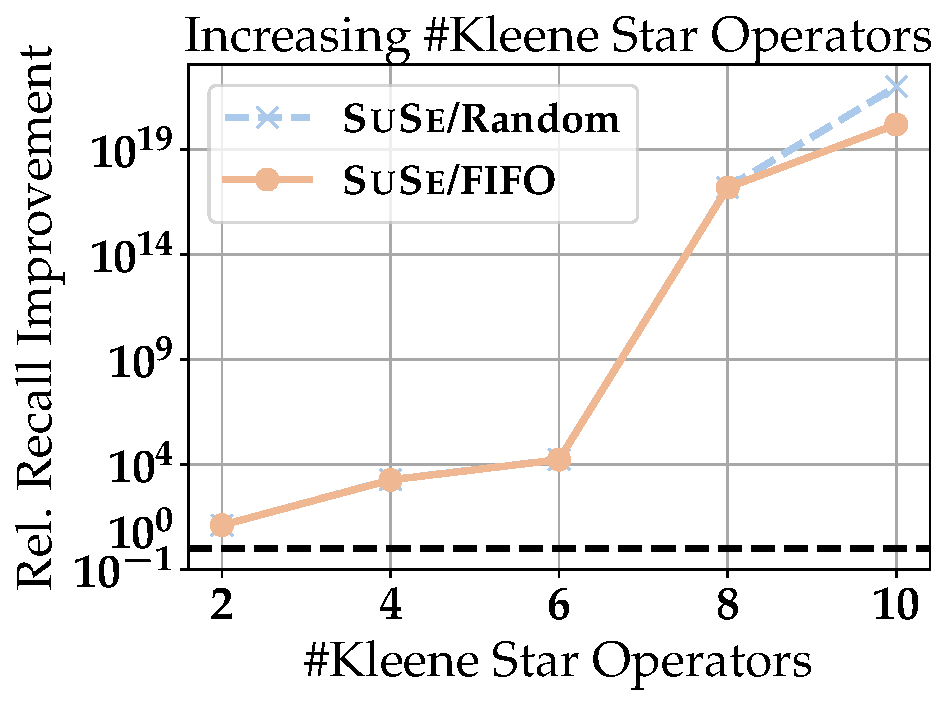
\includegraphics[width=\linewidth]{../runs/sensitivity_analysis/Figure8c_changing_number_of_kleene_operators/plots/number_of_kleene_operators_combined_plot.pdf}
		\vspace{-18pt}
		\caption{}
		\label{plot:number_of_kleenes}
	\end{subfigure}
	\hfill
	\begin{subfigure}{.38\linewidth}
		\centering
		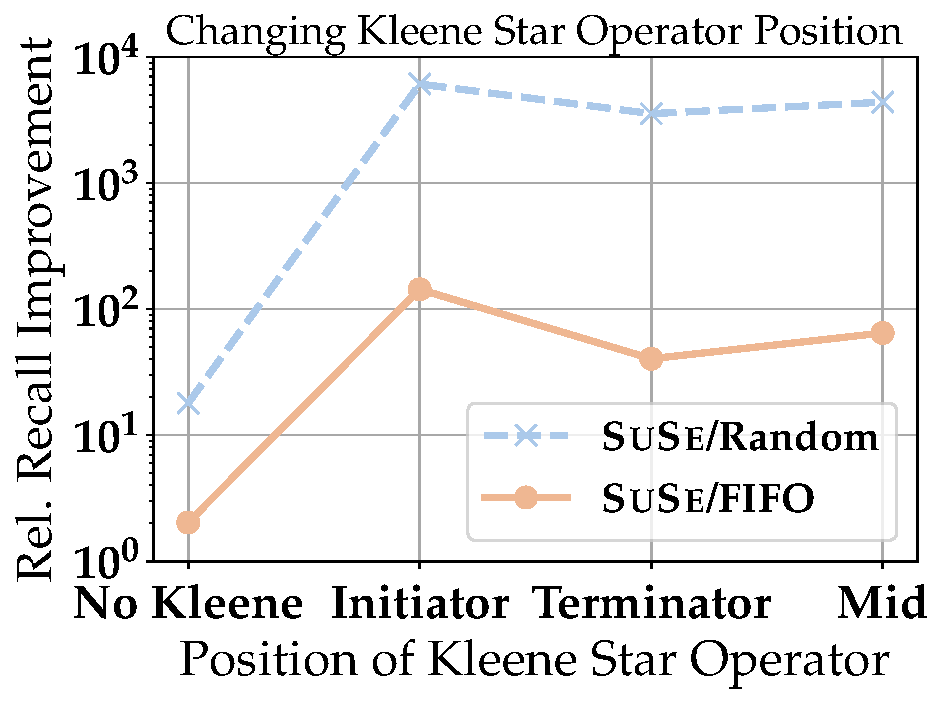
\includegraphics[width=\linewidth]{../runs/sensitivity_analysis/Figure8d_positional_kleene/plots/positional_kleene_plot.pdf}
		\vspace{-18pt}
		\caption{}
		\label{plot:positional_kleene}
	\end{subfigure}

	\vspace{1em} 
	\begin{subfigure}{.38\linewidth}
		\centering
		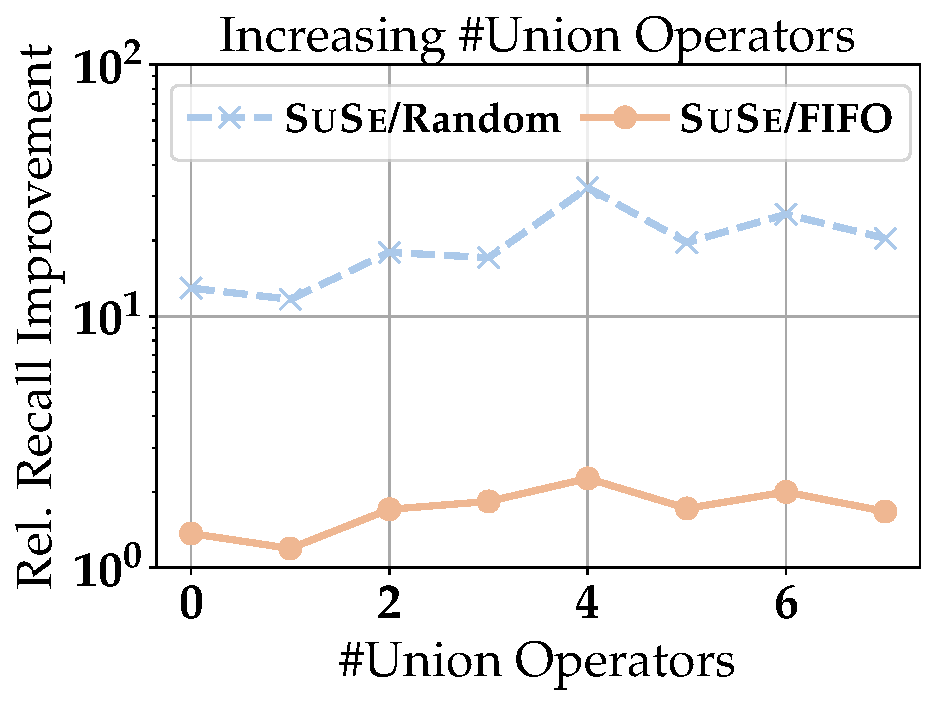
\includegraphics[width=\linewidth]{../runs/sensitivity_analysis/Figure8e_changing_number_of_disjunction_operators/plots/number_of_disjunction_operators_combined_plot.pdf}
		\vspace{-18pt}
		\caption{}
		\label{plot:number_of_unions}
	\end{subfigure}
	\hfill
	\begin{subfigure}{.38\linewidth}
		\centering
		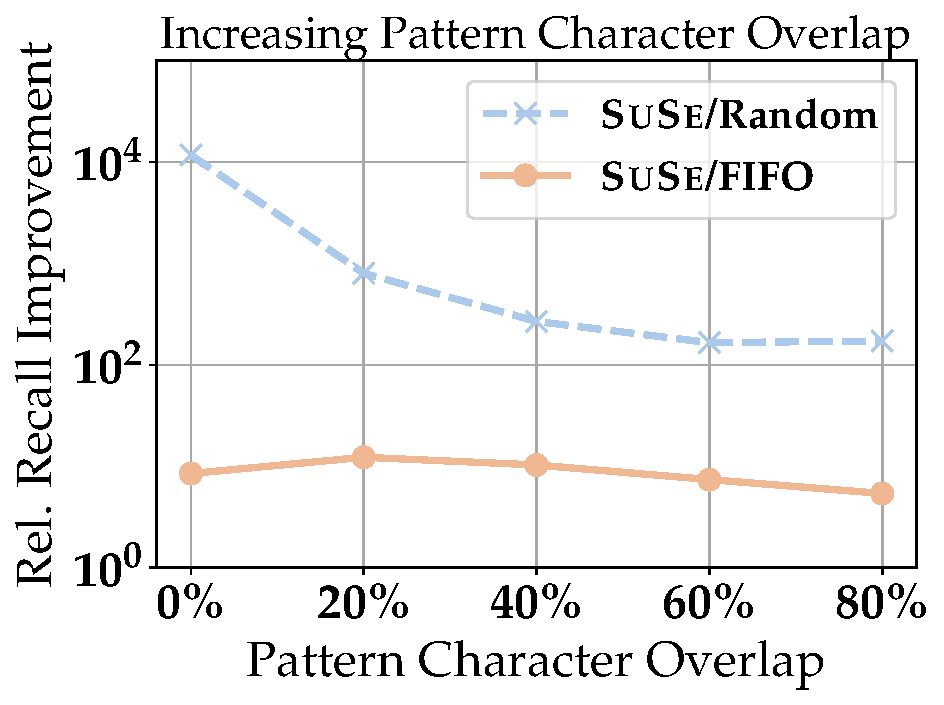
\includegraphics[width=\linewidth]{../runs/sensitivity_analysis/Figure8f_overlapping_characters/plots/disjunction_operator_overlapping_percentage.pdf}
		\vspace{-18pt}
		\caption{}
		\label{plot:query_character_overlap}
	\end{subfigure}

	\vspace{-1em}
	\caption{Examining the impact on relative recall improvement (higher is better) by varying (a) the number of evaluation timestamps $|\mathcal{E}|$, (b) the pattern length, (c) the count of Kleene stars, (d) Kleene star position, (e) union operator count, and (f) query character overlap.}
	\label{fig:operator_analysis}
	\vspace{-1em}
\end{figure*}


\subsection{Overall Effectiveness}
\label{subsec:overall-effectiveness}
We first compare against a random baseline (\suse{}/Random - S/R) and a FIFO
baseline (\suse{}/FIFO - S/F). In
\autoref{plot:summary_size_time_window_size} - \ref{plot:different_alphabet_probability_distributions}, we assessed how
variations in the summary size $|\mathcal{S}|$ ($100$ to $5000$),
time window size $q_\tau$ ($10$ to $250$), and
alphabet probability distribution $P_\Sigma$ (Zipfian, uniform (u), normal (n)) affect
the relative recall improvement, using a query with $q_\gamma = a(b^*c)^*d(e|f)g^*$.

\suse{} outperforms its baselines by choosing summaries that generate
up to $10^{20}$ more matches. There is no parameter combination, in which
\suse{}
performs worse than a baseline (black dashed line). A clear
trend emerges for both plots: the larger $q_\tau$ and the smaller
$|\mathcal{S}|$, the more significant the advantage.

As the summary size increases, the baselines find more matches by chance; nevertheless, for these parameters, \suse{} chooses stream subsequences that generate at least three orders of magnitude more matches on average.

\textbf{Ablation Study.} We compared \suse{}'s benefit function $\mathcal{B}$ against
a setup using solely the present benefit $\mathcal{B}_{\text{pres}}$, i.e.,
{denoted by $\mathcal{B}$/$\mathcal{B}_{\text{pres}}$}, in terms
of the relative recall improvement, the related absolute recall, and the detected
matches recall. %As before, we are varying $|\mathcal{S}|$ and $q_\tau$.
In \autoref{plot:ablation_study}, a trend similar to that in
\autoref{plot:summary_size_time_window_size} is observed: smaller
$|\mathcal{S}|$ and larger $q_\tau$ lead to better subsequence selections. This
is attributed to $\mathcal{B}$ providing a more accurate assessment of an element's future potential.

For $q_\tau = 250$, \suse{} with $\mathcal{B}$ obtains at least three orders of
magnitude more matches on average over solely using
$\mathcal{B}_{\text{pres}}$ and up to $10^{18}$ more for smaller values of
$|\mathcal{S}|$, showing the effectiveness of $\mathcal{B}$.

\textbf{Absolute Recall.} In \autoref{plot:average_total_match_ratio_recall_2000}, we evaluated the loss function $l_{\textsc{Count}}$ from \autoref{problem-definition}, showing how closely \suse{} approaches the optimal recall value.

Here, increasing $|\mathcal{S}|$ positively affects
recall. This
is attributed to the reduced difference between the ground
truth's summary size (equal to the stream size) and \suse{}'s summary size.
\suse{} clearly attains higher recall values when employing expected
benefits $\mathcal{B}$,
compared to using solely
$\mathcal{B}_{\text{pres}}$. Also, when
$|\mathcal{S}| \geq q_\tau$, with $\mathcal{B}$, \suse{} selects
substantially better subsequences, increasing recall by
up to $80\%-95\%$. This trend can be attributed to our assumption in
\autoref{subsec:selection-strategy} regarding the expected benefit
$\mathcal{B}$, where we implicitly assumed

that at least one time window size of elements fits into the summary. For
values $|\mathcal{S}| \geq q_\tau$, this assumption is valid, leading to more
accurate estimates and an enhanced recall.


\textbf{Detected Matches Recall.} For
\autoref{plot:detected_matches_recall_2000}, we examined how many of \emph{all}
possible matches were present in \suse{}, again comparing $\mathcal{B}$ and
$\mathcal{B}_{\text{pres}}$. The trends align closely with those observed for
the absolute recall. \suse{} with $\mathcal{B}$ yields a recall
of $90\%-98\%$ for $|\mathcal{S}| = 500$, indicating that \suse{}
chooses rich stream subsequences.

\subsection{Sensitivity Analysis}
\label{subsec:sensitivity-analysis}
Next, we assess the effect of various parameters on the relative recall
improvement. We fix $q_\tau = 100$ and $|\mathcal{S}| = 500$, and vary
stream sizes ($10000$ - $25000$), the numbers of evaluations
($25$ - $50$), and $P_\Sigma$ (Zipfian or uniform). We report
averages of over $50$ runs.

\textbf{Number of Evaluation Timestamps.}
\autoref{plot:evaluation_timestamps} examines the influence of increasing the number of evaluation timestamps $|\mathcal{E}|$ on the relative recall improvement. As the boxplots indicate, increasing the number of evaluations does not impact the results.

\textbf{Pattern Length.} \autoref{plot:query_length} shows that as the pattern
length grows, selecting
subsequences that yield matches becomes increasingly challenging.

\suse{} addresses this by quantifying the importance of individual elements,
prioritizing, for instance, rare elements that are essential to keep to obtain
matches.

While for pattern length two, FIFO performs slightly better, for pattern
lengths above ten, \suse{} is superior by up to almost five
orders of magnitude.

\textbf{Kleene Operator.} %To explore the impact of Kleene operators,
In \autoref{plot:number_of_kleenes}, we employed a regular expression of length twelve and
incrementally increased the number of Kleene operators, distributing them
randomly. As \suse{} is aware of characters with Kleene
operators (by \textsc{Count}/\textsc{Sum} rules), it selects better
summaries.

In \autoref{plot:positional_kleene}, we examined four regular expressions: one
without a Kleene operator and three with the Kleene's position varied.
Without Kleene, \suse{}'s advantages are minimal, while there is a
large difference for the other cases, independent of the Kleene position.

\textbf{Union Operator.} We also
explored the effect of the union operator in
\autoref{plot:number_of_unions}. We varied the number of
unions from zero to seven and generated and combined random sequences for $q_\gamma$'s with union operators. Yet, the impact is negligible.

In \autoref{plot:query_character_overlap}, we fixed a query of length ten and
progressively increased the character overlap. We randomly selected two
characters of the given query for each step, linking them to the query and a
union.

While the baselines show different trends, in all configurations, \suse{}
yields significant improvements.


\subsection{Efficiency}
\label{subsec:efficiency}
\textbf{\textsc{StateSummary} State-of-the-art Comparison.} {We compared \textsc{StateSummary}'s efficiency
against the state-of-the-art RegEx engine REmatch and two CEP engines,
FlinkCEP and CORE, in \autoref{fig:suse_vs_rematch}. {We summarize the idea
of the experiment as follows: To assess the current state, i.e., the current
number of matches and involvements of individual events, we would need to
use a RegEx/CEP engine. However, such engines implement a traditional
two-step approach: first building the state, then evaluating aggregate
functions over it.} Hence, these methods deliver matches and
exact results. In contrast, our approach avoids the direct maintenance
of (partial) matches and evaluates aggregate functions without match
materialization. When the summary is smaller than the word to process, the
resulting aggregate value is approximate; however, if the summary is greater
than or equal to the word size, the results remain exact.

Given the inferior performance of other RegEx engines
(see~\cite{Riveros2023}) {and their limitation in computing \emph{all}
subsequence matches}, we focus on REmatch as a representative RegEx engine.

FlinkCEP is an industry-strength tool offering a
robust framework for fault-tolerant and distributed stream processing. As
such, it offers features that are not implemented in the other engines,
which induces a non-negligible overhead during query evaluation that needs
to be considered in any comparative analysis. We note for FlinkCEP, though,
that parallelizing the workload is not straightforward, since the input
stream must be keyed and partitioned while ensuring that \emph{all} matches
are found, which is further complicated by operators like Kleene star.}
While FlinkCEP employs a traditional automata-based evaluation, CORE employs
compact match representations, avoiding exponential state growth, and
provides match enumeration with output-linear delay.

\begin{figure}[t]
	\begin{subfigure}{.38\linewidth}
		\centering
		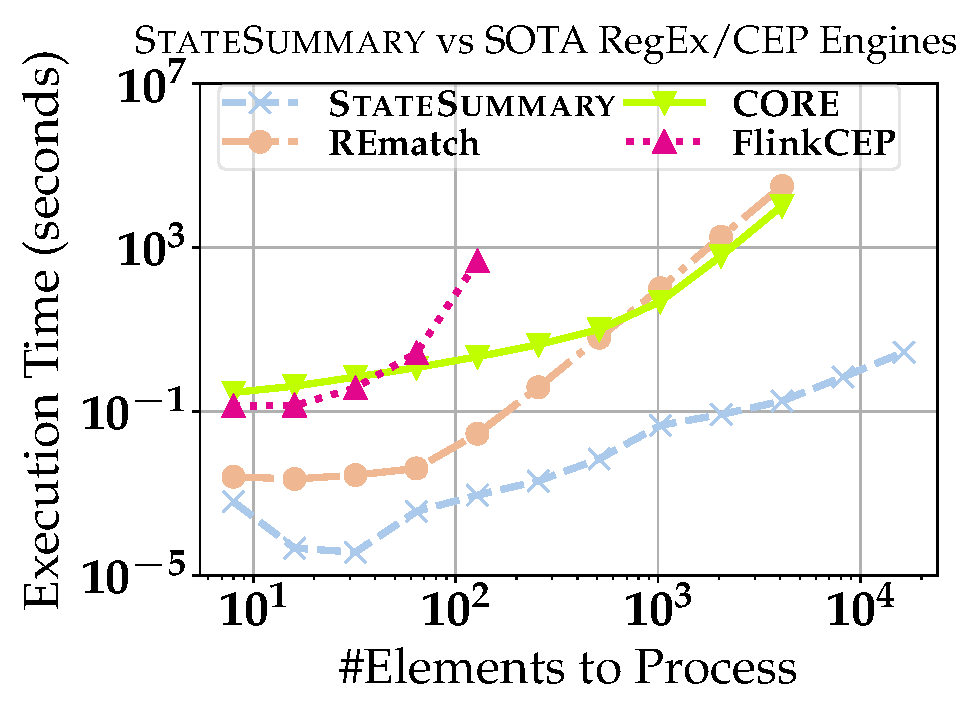
\includegraphics[width=1.0\linewidth]{../runs/efficiency/Figure9a_suse_vs_rematch_vs_core_vs_flinkcep/plots/suse_vs_rematch_vs_core_vs_flinkcep.pdf}
		\vspace{-18pt}
		\caption{}
		\label{plot:suse-vs-rematch-exec-time}
	\end{subfigure}
    \hfill
	\begin{subfigure}{.38\linewidth}
		\centering
		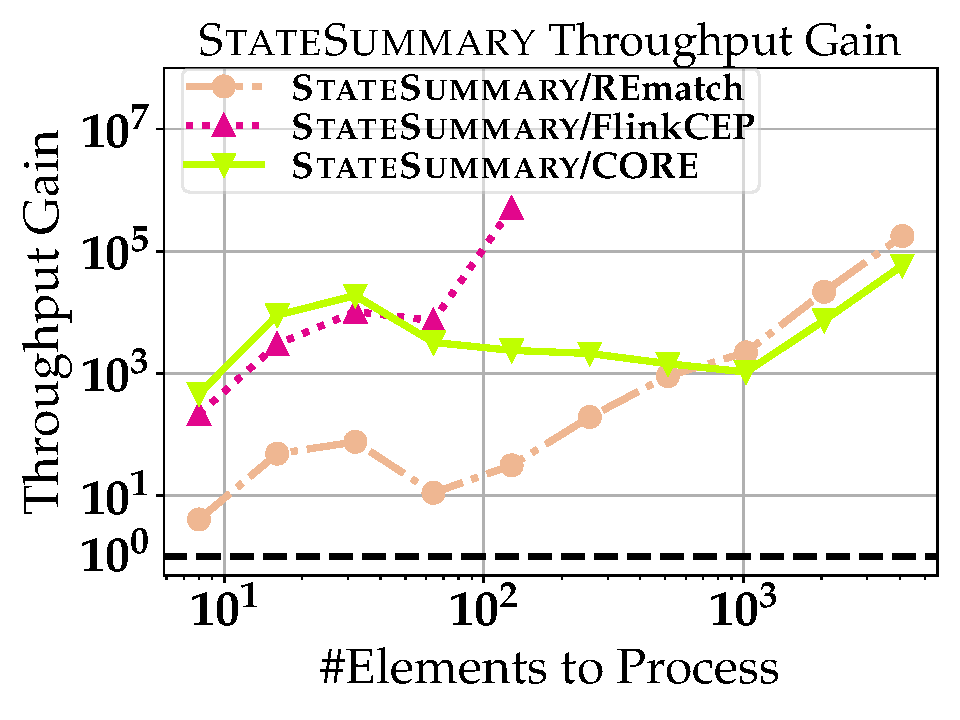
\includegraphics[width=1.0\linewidth]{../runs/efficiency/Figure9b_throughput_gain_over_rematch_core_flinkcep/plots/throughput_gain_over_rematch_core_flinkcep.pdf}
		\vspace{-18pt}
		\caption{}
		\label{plot:suse-vs-rematch-throughput-gain}
	\end{subfigure}
	\vspace{-1em}
    \hfill
    \caption{Comparison against the state of the art, focusing on (a)
    execution time (lower is better) and (b) throughput gain (higher is
    better), varying the number of processed elements.}
	\label{fig:suse_vs_rematch}
	\vspace{-1em}
\end{figure}

\begin{figure*}[t]
	\centering
	\begin{subfigure}{.38\linewidth}
		\centering
		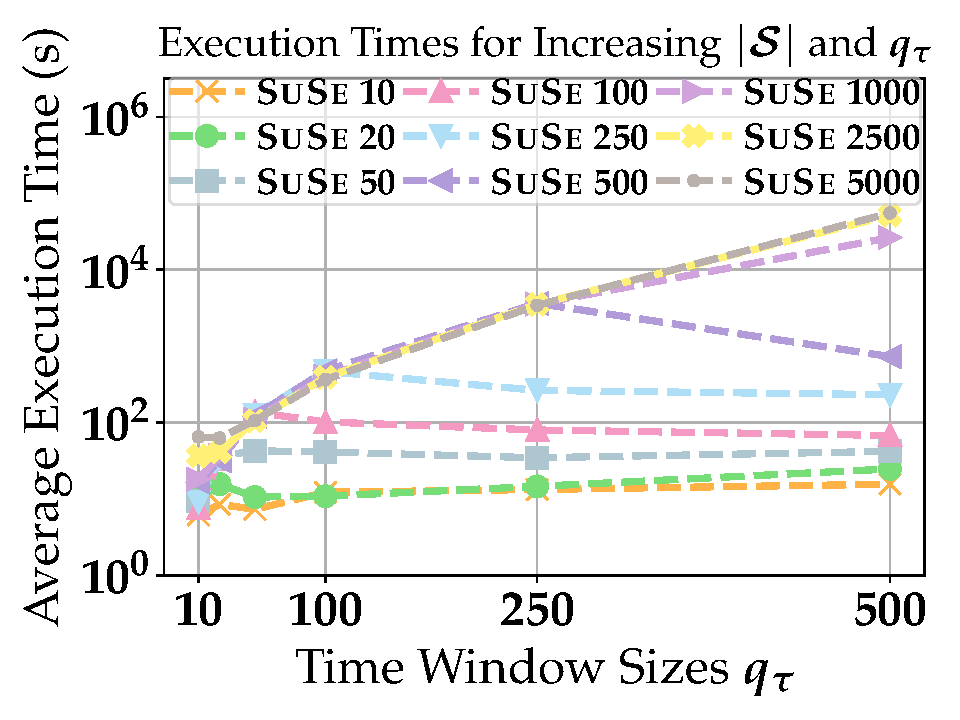
\includegraphics[width=\linewidth]{../runs/efficiency/Figure10a_execution_time_summary_time_window_comparison/plots/execution_time_summary_time_window_comparison.pdf}
		\vspace{-18pt}
		\caption{}
		\label{plot:execution_time_plot}
	\end{subfigure}
	\hfill
	\begin{subfigure}{.38\linewidth}
		\centering
		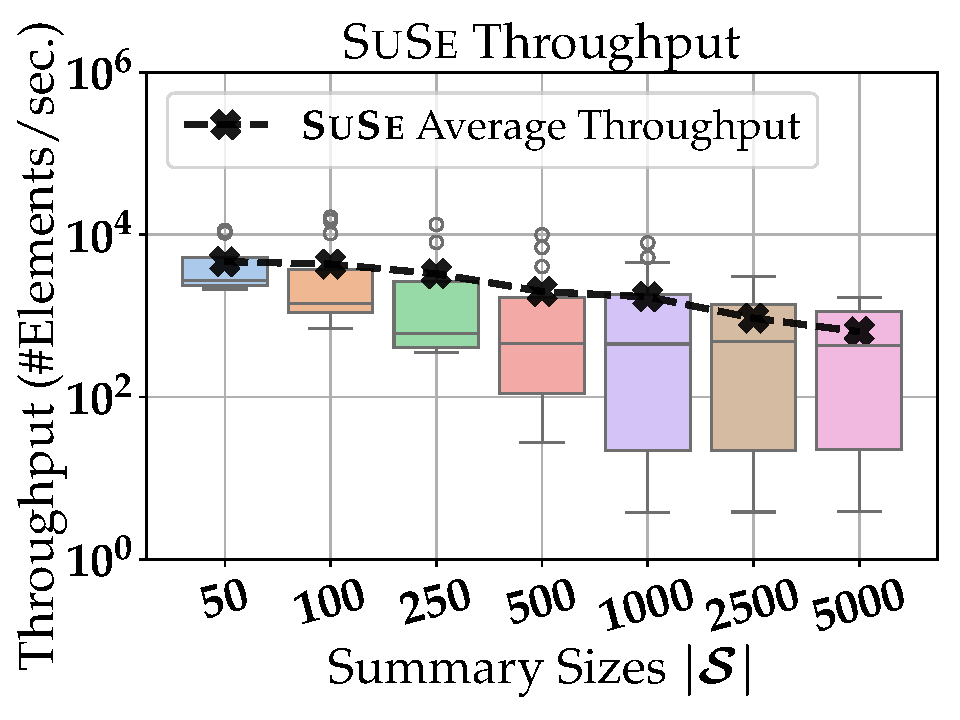
\includegraphics[width=\linewidth]{../runs/efficiency/Figure10b_throughput_boxplot/plots/throughput_boxplot.pdf}
		\vspace{-18pt}
		\caption{}
		\label{plot:execution_throughput}
	\end{subfigure}

	\vspace{1em} 
    
	\begin{subfigure}{.38\linewidth}
		\centering
		\includegraphics[width=\linewidth]{../runs/efficiency/Figure10c_latency_boxplot/plots/latency_boxplot.pdf}
		\vspace{-18pt}
		\caption{}
		\label{plot:execution_latency}
	\end{subfigure}
	\hfill
	\begin{subfigure}{.38\linewidth}
		\centering
		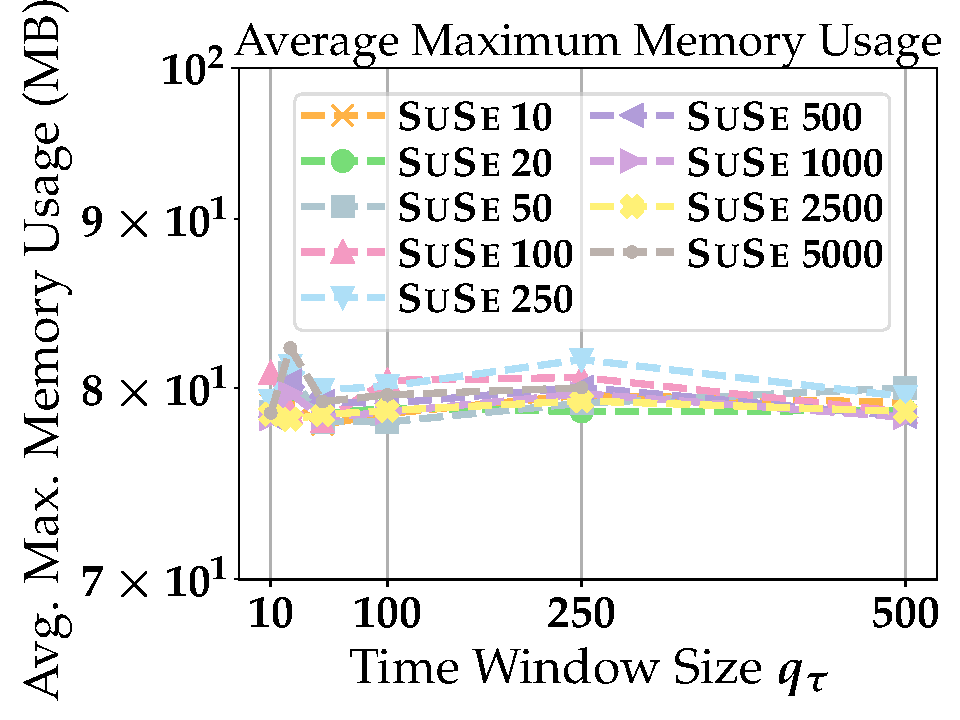
\includegraphics[width=\linewidth]{../runs/efficiency/Figure10d_memory_experiment/plots/average_maximum_memory_usage.pdf}
		\vspace{-18pt}
		\caption{}
		\label{plot:execution_memory_usage}
	\end{subfigure}

	\vspace{-1em}
	\caption{(a) Execution time (lower is better) for processing $10^5$ elements across different summary and time window sizes, (b) throughput (higher is better), (c) average minimum, average maximum, and average processing latency per element (lower is better), and (d) average maximum memory usage (lower is better).}
	\label{fig:exeuction_time_throughput_latency_memory}
	\vspace{-1em}
\end{figure*}

The evaluated procedures utilized one to two cores on
average (i.e., FlinkCEP did not parallelize processing as the input stream
is not keyed). The maximum resident set size was $\approx500$ MB for
FlinkCEP (increasing to over $1$ GB for $x = 256$, and not terminating after
several hours), $\approx409$ MB for CORE, $\approx 3.3$ MB for REmatch, and
$\approx 81$ MB for \suse{}.

{{We set the summary size to the corresponding $x$-value, ensuring that the
processed word fits entirely within the summary. Thus, we focused
exclusively on \textsc{StateSummary} operations without employing summary
selection, computing exact values instead of approximations. We set the time
window size such that all elements fit into a single window, maximizing the
number of matches to be detected. Also, we ensured that all methods produced
the same result when evaluating the aggregate function.} We tested with
$q_\gamma = ABCD$ (the REmatch syntax being
$!x\{A\}.*!y\{B\}.*!z\{C\}.*!w\{D\}$) for the required processing time of
input words of varying sizes. As input, we choose words of the form
$A^iB^iC^iD^i$ with $i \in \mathbb{N}^+$, e.g., $A^8B^8C^8D^8$, ensuring an increase in matches for rising $x$-values.}

{\textsc{StateSummary} consistently processes words at least an order of magnitude faster than REmatch, and at least three orders of magnitude faster than CORE and Flink. Particularly for words longer than $512$ characters, the performance gap between \textsc{StateSummary} and both REmatch and CORE significantly widens, while Flink did not terminate for these values due to overload.}


The performance differences induce throughput gains, as shown in
\autoref{plot:suse-vs-rematch-throughput-gain}. The ratio indicates how much
more quickly \textsc{StateSummary} processed a word than REmatch, CORE, or Flink. The throughput gain always exceeds one, indicating \textsc{StateSummary}'s superiority; for longer words, this gain increases significantly.


\textbf{\suse{}'s Overall Efficiency.} In
\autoref{fig:exeuction_time_throughput_latency_memory}, we examined how varying
$|\mathcal{S}|$ (see legend) and $q_\tau$ affects the execution time,
throughput, processing latency per element, and memory usage of \suse{} (employing summary selection) for processing a stream of $10^5$ elements.
 \autoref{plot:execution_time_plot} shows that

 the larger $|\mathcal{S}|$ and the larger $q_\tau$, the longer the execution
 time.
Also, a time window size exists for all
 procedures up to a summary size of $500$, where execution time stabilizes
 or slightly decreases. The reasoning being that the \textsc{Remove}
 operation is the most
 expensive one (see \autoref{subsec:summary-operations}), with cost
 $min(q_\tau,
 |\mathcal{S}|)$. Once either $|\mathcal{S}| > q_\tau$ or $q_\tau >
 |\mathcal{S}|$, the smaller value of the two parameters becomes the limiting
 factor for runtime, rendering the influence of the other parameters
 marginal. %, which can also be observed in the results. In addition,
 With larger $q_\tau$, \suse{} chooses better subsequences, which reduces
 the number of \textsc{Remove} operations and explains the drop in
 runtime for $q_\tau \geq |\mathcal{S}|$.

In \autoref{plot:execution_throughput}, we examined the resulting throughput
values for a fixed $q_\tau = 500$.

For the same reasons as discussed above,
there is a decline in throughput as the summary size expands.


In \autoref{plot:execution_latency}, we investigated the resulting average
min, max, and average processing latency per element per second.
A boxplot shows the latencies for increasing $q_\tau$, while the
corresponding line plots denote the averages. A larger
$|\mathcal{S}|$ leads to
elevated processing latencies. However, the median of the
average processing latencies consistently remains below $10^{-1}s$, showing streaming feasibility.


Finally, the induced memory footprint turned out to be negligible and
constant for various $|\mathcal{S}|$ and $q_\tau$, see
\autoref{plot:execution_memory_usage}.

\begin{figure*}[t]
	\centering
	\begin{subfigure}{.32\linewidth}
		\centering
		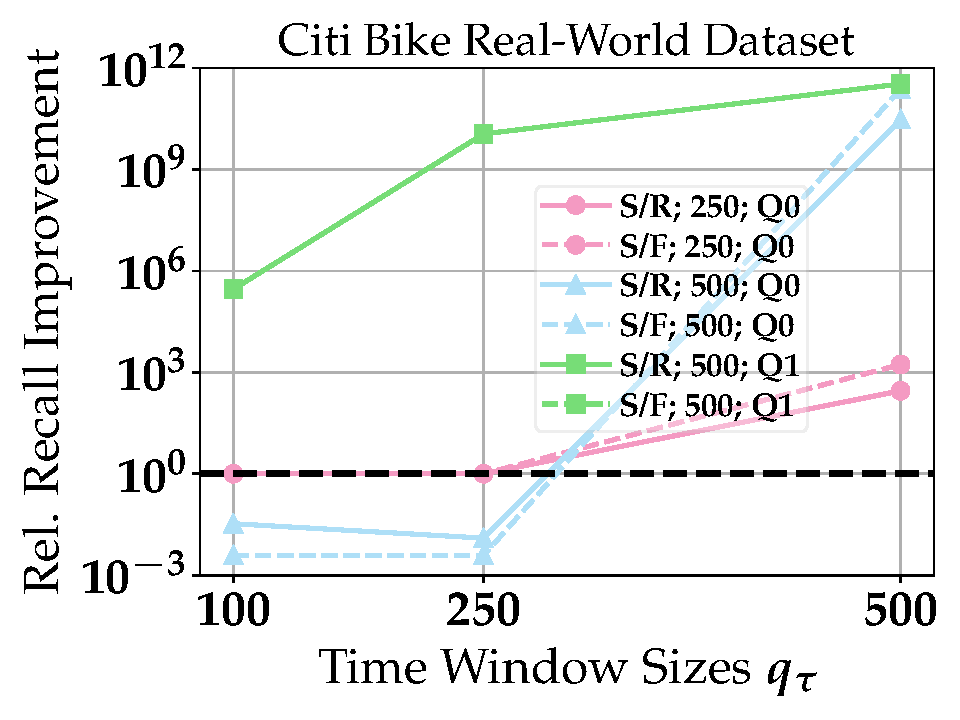
\includegraphics[width=1.0\linewidth]{../runs/real_world_experiments/Figure11a_CitiBike_queries/plots/CitiBike_queries.pdf}
		\vspace{-18pt}
		\caption{}
		\label{plot:citi_bike_average_total_match_ratio}
	\end{subfigure}
	\hfill
	\begin{subfigure}{.32\linewidth}
		\centering
		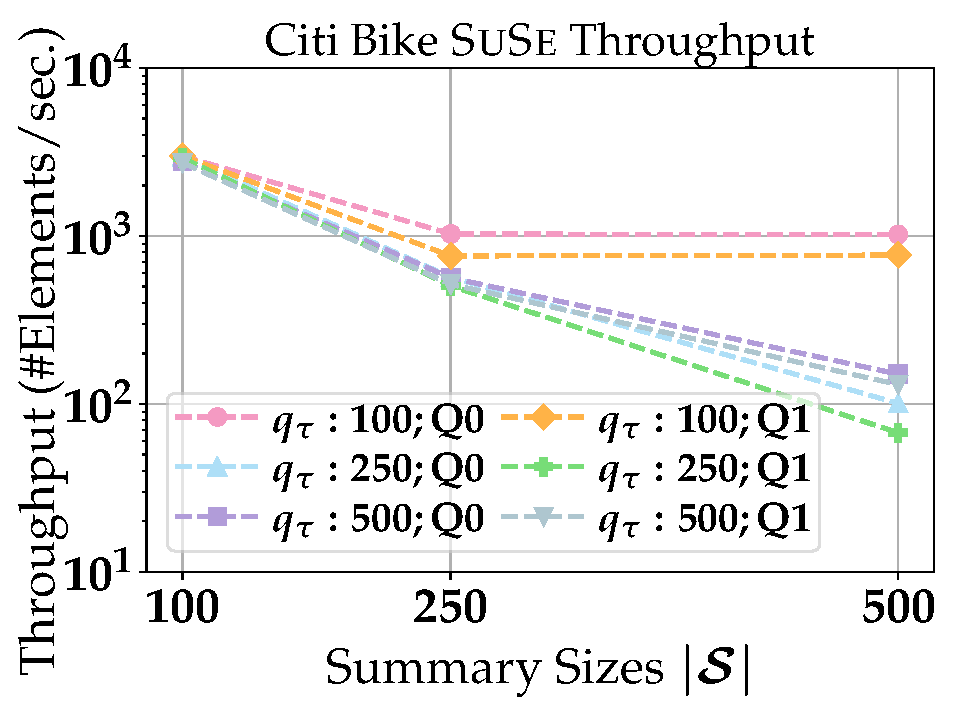
\includegraphics[width=1.0\linewidth]{../runs/real_world_experiments/Figure11b_CitiBike_throughput_lineplot/plots/CitiBike_throughput_lineplot.pdf}
		\vspace{-18pt}
		\caption{}
		\label{plot:citi_bike_throughput}
	\end{subfigure}
	\hfill
	\begin{subfigure}{.32\linewidth}
		\centering
		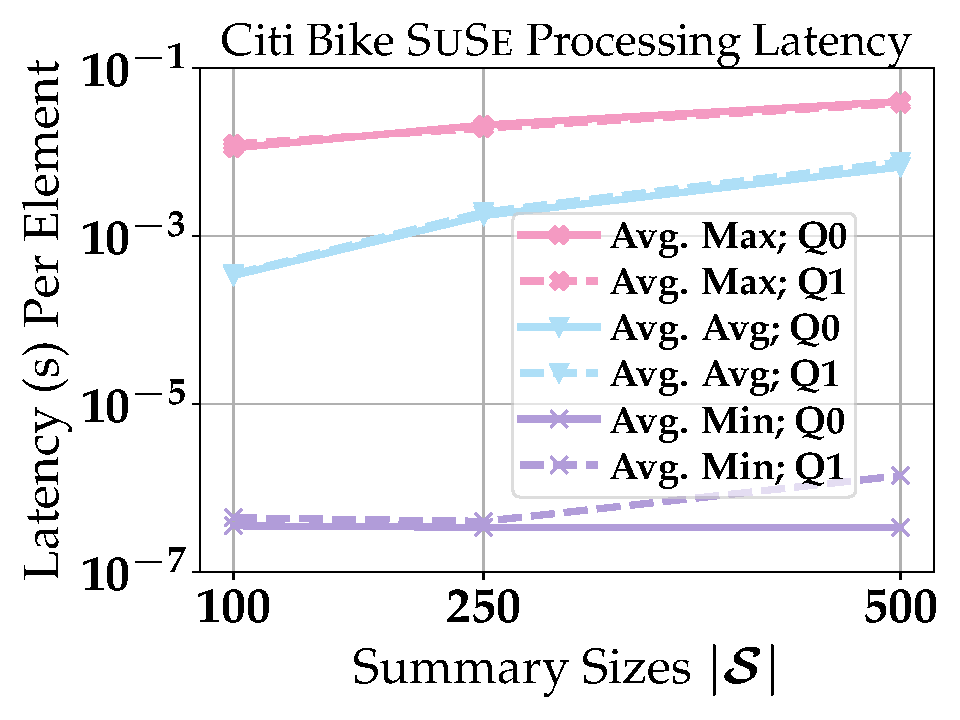
\includegraphics[width=1.0\linewidth]{../runs/real_world_experiments/Figure11c_CitiBike_latency_lineplot/plots/CitiBike_latency_lineplot.pdf}
		\vspace{-18pt}
		\caption{}
		\label{plot:citi_bike_latency}
	\end{subfigure}
	\vspace{-1em}
	\caption{Citi Bike: (a) relative recall improvement (higher is better), (b) throughput (higher is better), and (c) latency (lower is better).}
	\label{fig:citi_bike}
	\vspace{-1em}
\end{figure*}

\subsection{Case Study: Citi Bike}
\label{subsec:citibike}
\textbf{Character Types and Queries.} \autoref{fig:citi_bike} denotes our
results for the Citi Bike real-world dataset. The character types encompass
rides on frequented routes, pinpoint brief rides at busy stations, rides at
central stations, and member rides at quieter stations, giving a thorough
understanding of the Citi Bike dynamics. We defined a query with $Q0_\gamma =
E(H|K)^*E$, recognizing patterns where a ride starts at a busy station, followed by a combination of rides at central and quieter stations, ending with a ride at a busy station, suggesting probable areas for station enhancements or
upkeep. The second query, $Q1_\gamma = (E|B|F)^+CEHF$, captures sequences of
rides that start at busy stations, popular routes, or extended rides at central
spots, followed by short and consecutive rides at busy stations, a trip at a
central location, and concluding with a prolonged ride there.

\textbf{Effectiveness.} To examine the relative recall improvement, we varied
$|\mathcal{S}|$ and $q_\tau$ in
\autoref{plot:citi_bike_average_total_match_ratio}. For both queries, not all
summary sizes yielded matches. Generally,
there is an upward trend in the results with a larger
$q_\tau$; \suse{} identifies subsequences that are between three
and twelve orders of magnitude superior for $q_\tau = 500$.

\textbf{Throughput and Latency.} Throughput and
latency of \suse{} are shown in \autoref{plot:citi_bike_throughput} and
\autoref{plot:citi_bike_latency}. 
For smaller values of $|\mathcal{S}|$ and $q_\tau$ (refer to legend), \suse{}'s
throughput increases. 
However, with larger values for $|\mathcal{S}|$ and $q_\tau$, the lower
throughput is

attributed to the \textsc{Remove} operation.
\autoref{plot:citi_bike_latency} shows the avg min, avg max, and avg
latency of \suse{}, with $q_\tau = 500$. An increase in summary size leads to
higher latencies. Yet, the average max latency hovers around $10^{-2}$
seconds, while the average processing latency remains under $10^{-2}$ seconds
for $|\mathcal{S}| = 500$, which meets real-time demands.


\begin{figure*}[t]
	\centering
	\begin{subfigure}{.32\linewidth}
		\centering
		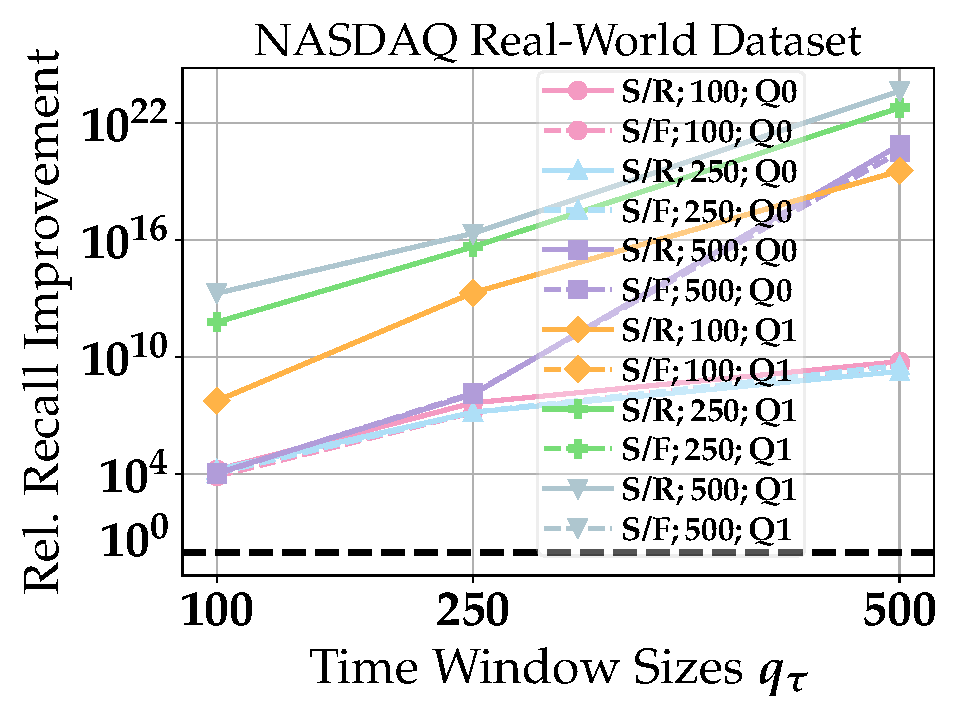
\includegraphics[width=1.0\linewidth]{../runs/real_world_experiments/Figure12a_NASDAQ_queries/plots/NASDAQ_queries.pdf}
		\vspace{-15pt}
		\caption{}
		\label{plot:nasdaq_average_total_match_ratio}
	\end{subfigure}
	\begin{subfigure}{.32\linewidth}
		\centering
		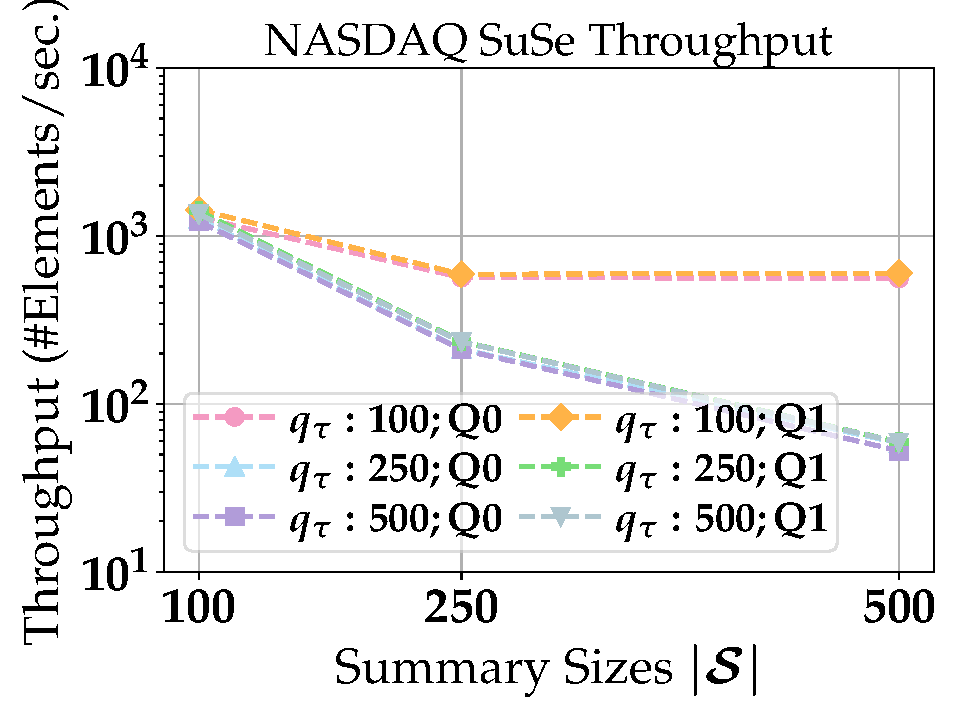
\includegraphics[width=1.0\linewidth]{../runs/real_world_experiments/Figure12b_NASDAQ_throughput_lineplot/plots/NASDAQ_throughput_lineplot.pdf}
		\vspace{-15pt}
		\caption{}
		\label{plot:nasdaq_throughput}
	\end{subfigure}
	\begin{subfigure}{.32\linewidth}
		\centering
		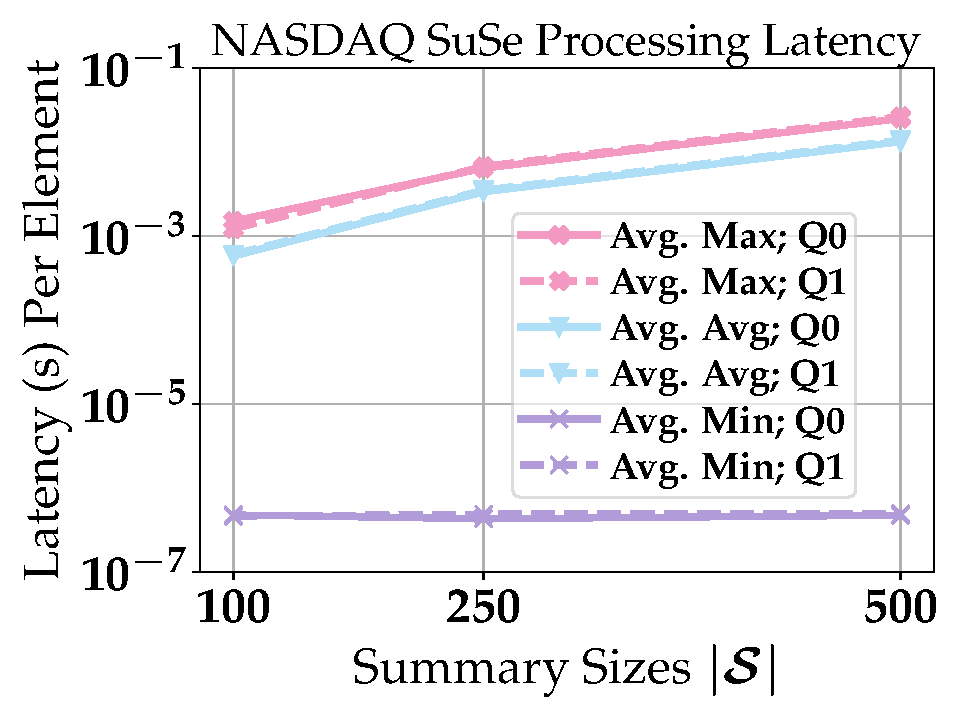
\includegraphics[width=1.0\linewidth]{../runs/real_world_experiments/Figure12c_NASDAQ_latency_lineplot/plots/NASDAQ_latency_lineplot.pdf}
		\vspace{-15pt}
		\caption{}
		\label{plot:nasdaq_latency}
	\end{subfigure}
    \vspace{-1em}
	\caption{NASDAQ: (a) relative recall improvement (higher is better), (b) throughput (higher is better), and (c) latency (lower is better).}
	\label{fig:nasdaq}
	\vspace{-1em}
\end{figure*}
